% -*- TeX -*-
%
% ----------------------------------------------------------------------
%
%                           Brad T. Aagaard
%                        U.S. Geological Survey
%
% {LicenseText}
%
% ----------------------------------------------------------------------
%
\documentclass[pdftex,cig,slideColor]{pp4slides}
\usepackage{amsmath}
\usepackage{array}
\usepackage{xspace}
\usepackage{multirow}
\usepackage{ulem}

\newcommand{\newfeature}[1]{{\color{blue}#1}}

\title{PyLith 1.4 Tutorial}
\subtitle{}
\author{Brad Aagaard\\[10pt]
  Charles Williams and Matthew Knepley}
\institution{\includegraphics[height=2cm]{../../logos/cig}}
\date{June 22, 2009}

% --------------------------------------------------------- DOCUMENT
\begin{document}

\bgadd{\vspace*{7.9in}%
  \begin{center}%
    \includegraphics[height=14mm]{../../logos/cig}
  \end{center}}

% ------------------------------------------------------------ SLIDE
\foilhead{Crustal Deformation Modeling}
  \summary{Overview of workflow for typical research problem}

  \vfill
  \begin{center}
    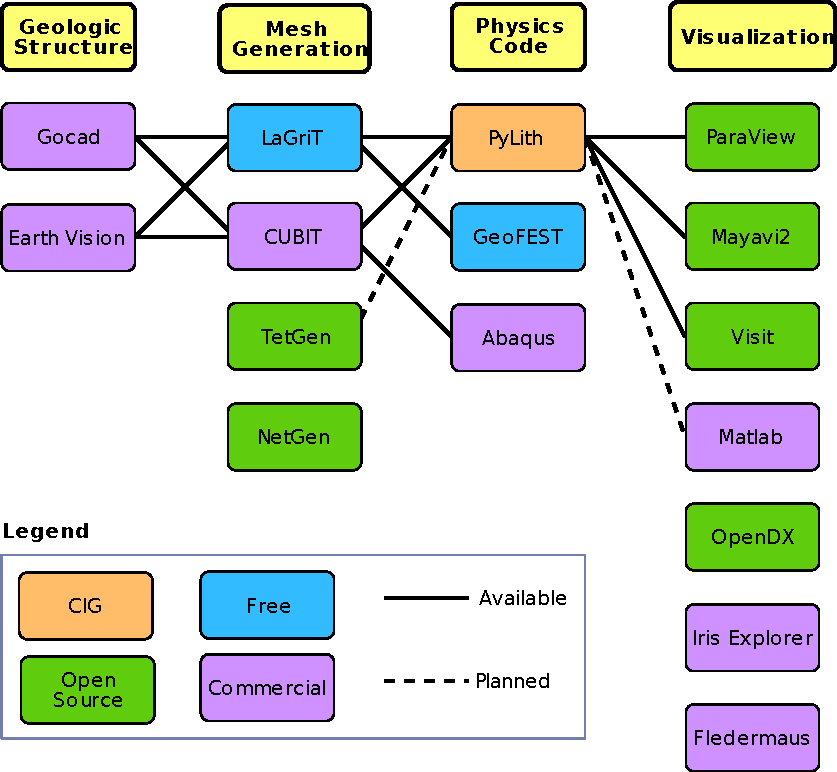
\includegraphics[scale=1.15]{figs/workflow}
  \end{center}
  \vfill

% ------------------------------------------------------------ SLIDE
\foilhead{Ingredients for Running PyLith}

  \begin{itemize}
  \item Simulation parameters
  \item Finite-element mesh
    \begin{itemize}
    \item Mesh exported from LaGriT
    \item Mesh exported from CUBIT
    \item Mesh constructed by hand (PyLith mesh ASCII format)
    \end{itemize}
  \item Spatial databases for physical properties, boundary
    conditions, and rupture parameters
    \begin{itemize}
    \item SCEC CVM-H or USGS Bay Area Velocity model
    \item Simple ASCII files
    \end{itemize}
  \end{itemize}

% ------------------------------------------------------------ SLIDE
\foilhead{Spatial Databases}
  \summary{User-specified field/value in space}

  \begin{itemize}
 \item Examples
    \begin{itemize}
    \item Uniform value for Dirichlet (0-D)
    \item Piecewise linear variation in tractions for Neumann BC (1-D)
    \item SCEC CVM-H seismic velocity model (3-D)
    \end{itemize}
  \item Generally independent of discretization for problem
  \item Available spatial databases
    \begin{description}
    \item[UniformDB] Optimized for uniform value
    \item[SimpleDB] Simple ASCII files (0-D, 1-D, 2-D, or 3-D)
    \item[SCECCVMH] SCEC CVM-H seismic velocity model v5.3
    \item[ZeroDispDB] Special case of UniformDB
    \end{description}
 \end{itemize}

  % ------------------------------------------------------------ SLIDE
\foilhead{Features in PyLith 1.4}
  \summary{Enhancements and new features in \newfeature{blue}}

  \begin{itemize}
  \item Time integration schemes
    \begin{itemize}
    \item Implicit time stepping for quasi-static problems
    \item Explicit time stepping for dynamic problems
    \end{itemize}
  \item Bulk constitutive models
    \begin{itemize}
    \item Elastic model (1-D, 2-D, and 3-D)
    \item Linear and Generalized Maxwell viscoelastic models (3-D)
    \item \newfeature{Power-law viscoelastic model (3-D)}
    \end{itemize}
  \item Boundary and interface conditions
    \begin{itemize}
    \item \newfeature{Time-dependent Dirichlet boundary conditions}
    \item \newfeature{Time-dependent Neumann (traction) boundary conditions}
    \item Absorbing boundary conditions
    \item Kinematic (prescribed slip) fault interfaces w/multiple ruptures
    \item \newfeature{Time-dependent point forces}
    \item Gravitational body forces
    \end{itemize}
  \end{itemize}

% ------------------------------------------------------------ SLIDE
\foilhead{Features in PyLith 1.4 (cont.)}
  \summary{Enhancements and new features in \newfeature{blue}}

  \begin{itemize}
  \item Automatic and user-controlled time stepping
  \item Ability to specify initial stress state
  \item Importing meshes
    \begin{itemize}
    \item LaGriT: GMV/Pset
    \item CUBIT: Exodus II
    \item ASCII: PyLith mesh ASCII format (intended for toy problems only)
    \end{itemize}
  \item Output: VTK files
    \begin{itemize}
    \item Solution over volume
    \item Solution over surface boundary
    \item State variables (e.g., stress and strain) for each material
    \item Fault information (e.g., slip and tractions)
    \end{itemize}
  \item \newfeature{Automatic conversion of units for all parameters}
  \end{itemize}

  % ------------------------------------------------------------ SLIDE
\foilhead{PyLith 1.4: Under-the-hood Improvements}
  \summary{}

  \begin{itemize}
  \item General cleanup of C++ code
  \item Pyrex/pyrexembed replaced by SWIG
    \begin{itemize}
    \item Greatly simplifies creating Python bindings for C++ objects
    \item SWIG generated files included in source distribution
    \item User-defined spatial databases and bulk constitutive models
    \end{itemize}
  \item Automatic nondimensionalization of problem
    \begin{itemize}
    \item User supplies pressure, time, and length scale of problem
    \item All parameters nondimensionalized appropriately
    \item Eliminates need to condition terms in sparse matrix
    \item Restores symmetry of sparse matrix (reduces memory use)
    \end{itemize}
  \item Integration with PETSc Scalable Nonlinear Equations Solvers
   \begin{itemize}
    \item Disp. increment formulation for implicit and dynamic time-stepping
   \end{itemize}
  \end{itemize}
    
% ------------------------------------------------------------ SLIDE
\foilhead{Time-Dependent Boundary Conditions}
  \summary{Dirichlet, Neumann, and Point Forces}
  
  \begin{equation*}
    \begin{split}
      f(\vec{x}) =& \\[10pt]
      & \begin{array}{lr}
        f_{0}(\vec{x}) + & \textrm{{\tt db\_initial}}\\[10pt]
        \dot{f}_{1}(\vec{x}) (t-t_{1}(\vec{x})) + & \textrm{{\tt db\_rate}}\\[10pt]
        f_{2}(\vec{x})a(t-t_{2}(\vec{x})) & \textrm{{\tt db\_change}}
      \end{array}
    \end{split}
  \end{equation*}
  \vfill
  \begin{description}
  \item[db\_initial] Initial value (constant in time)
  \item[db\_rate] Constant rate of change (spatially variable start time)
  \item[db\_change] Time history (spatially variable amplitude and
    start time)
  \end{description}
 
% ------------------------------------------------------------ SLIDE
\foilhead{PyLith as a Hierarchy of Components}
  \summary{Components are the basic building blocks}

  \vfill
  \begin{center}
    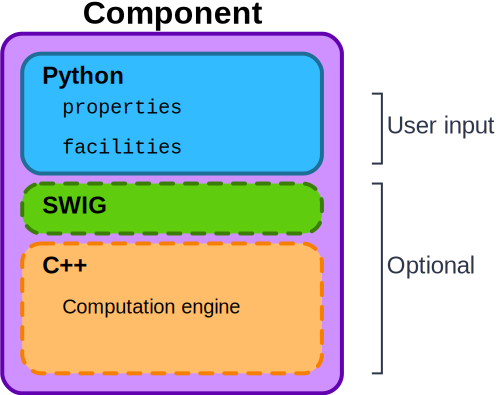
\includegraphics[scale=1.0]{figs/component}
  \end{center}  
  \vfill

% ------------------------------------------------------------ SLIDE
\foilhead{PyLith as a Hierarchy of Components}
  \summary{PyLith Application and Time-Dependent Problem}

  \vfill
  \begin{center}
    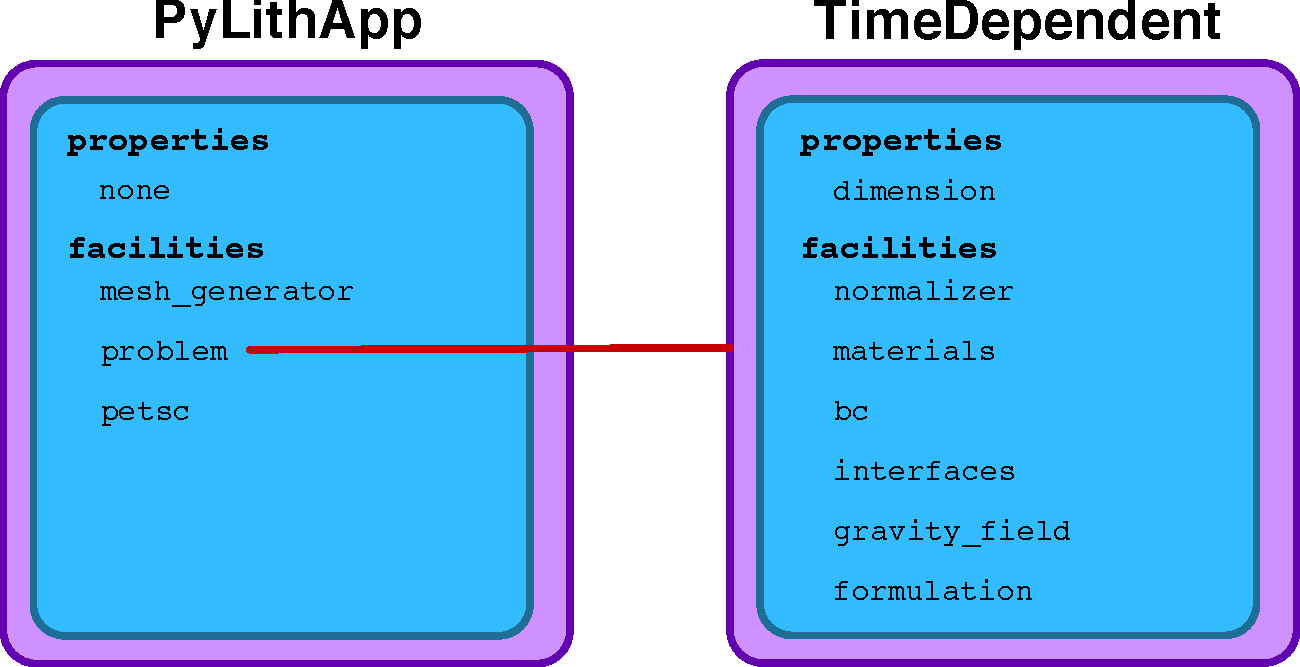
\includegraphics[scale=1.0]{figs/pylithapp}
  \end{center}  
  \vfill

% ------------------------------------------------------------ SLIDE
\foilhead{PyLith as a Hierarchy of Components}
  \summary{Fault with kinematic (prescribed slip) earthquake rupture}

  \vfill
  \begin{center}
    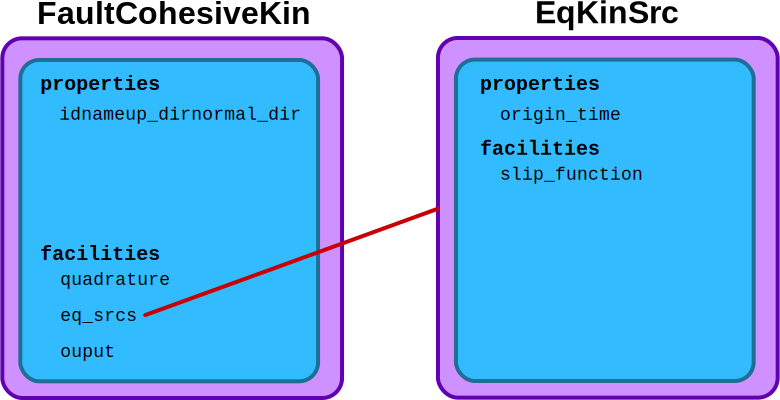
\includegraphics[scale=1.0]{figs/faultcohesivekin}
  \end{center}  
  \vfill

% ------------------------------------------------------------ SLIDE
\foilhead{PyLith Application Flow}
  \summary{}
 {\small
  \begin{minipage}[t]{3.75in}
    {\bf PyLithApp}\\[8pt]
    \begin{verbatim}
  main()
    mesher.create()
    problem.initialize()
    problem.run()
    \end{verbatim}
    \vspace*{20pt}
    {\bf TimeDependent (Problem)}\\[8pt]
    \begin{verbatim}
  initialize()
    formulation.initialize()

  run()
    while (t < totalTime)
      dt = formulation.getTimeStep()
      formulation.prestep()
      formulation.step()
      formulation.poststep()
\end{verbatim}
  \end{minipage}
  \hfill
  \begin{minipage}[t]{3.75in}
    {\bf Implicit (Formulation)}\\[8pt]
    \begin{verbatim}
  initialize()

  prestep()
    set constraints

  step()
    calculate residual
    solve for displacement increment

  poststep()
    update displacement field
    write output
\end{verbatim}
  \end{minipage}
}

% ------------------------------------------------------------ SLIDE
\foilhead{Ingredients for Running PyLith}

  \begin{itemize}
  \item Simulation parameters
    \begin{itemize}
    \item {\tt .cfg} ASCII files
    \item {\tt pylithapp.cfg} always read if it exists
    \item Command line arguments
    \end{itemize}
  \item Finite-element mesh
    \begin{itemize}
    \item Mesh exported from LaGriT
    \item Mesh exported from CUBIT
    \item Mesh constructed by hand (PyLith mesh ASCII format)
    \end{itemize}
  \item Spatial databases for physical properties, boundary
    conditions, and rupture parameters
  \end{itemize}

% ------------------------------------------------------------ SLIDE
\foilhead{Example: {\tt twocells/twoquad4 axialdisp.cfg}}
  \summary{Axial extension via prescribed displacements}

  \vfill
  \begin{center}
    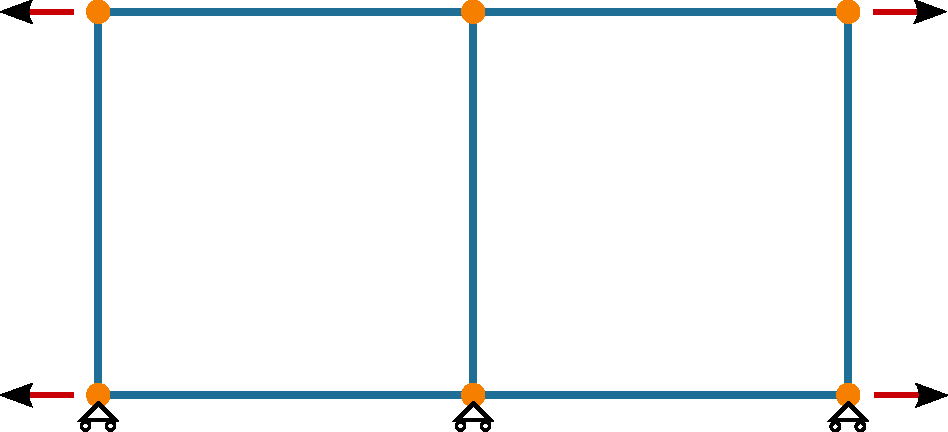
\includegraphics[scale=1.0]{figs/axialdisp_diagram}
  \end{center}
  \vfill

% ------------------------------------------------------------ SLIDE
\foilhead{\ }

\vspace*{-1.0in}%
{\large Example: {\tt twocells/twoquad4 axialdisp.cfg}}\\
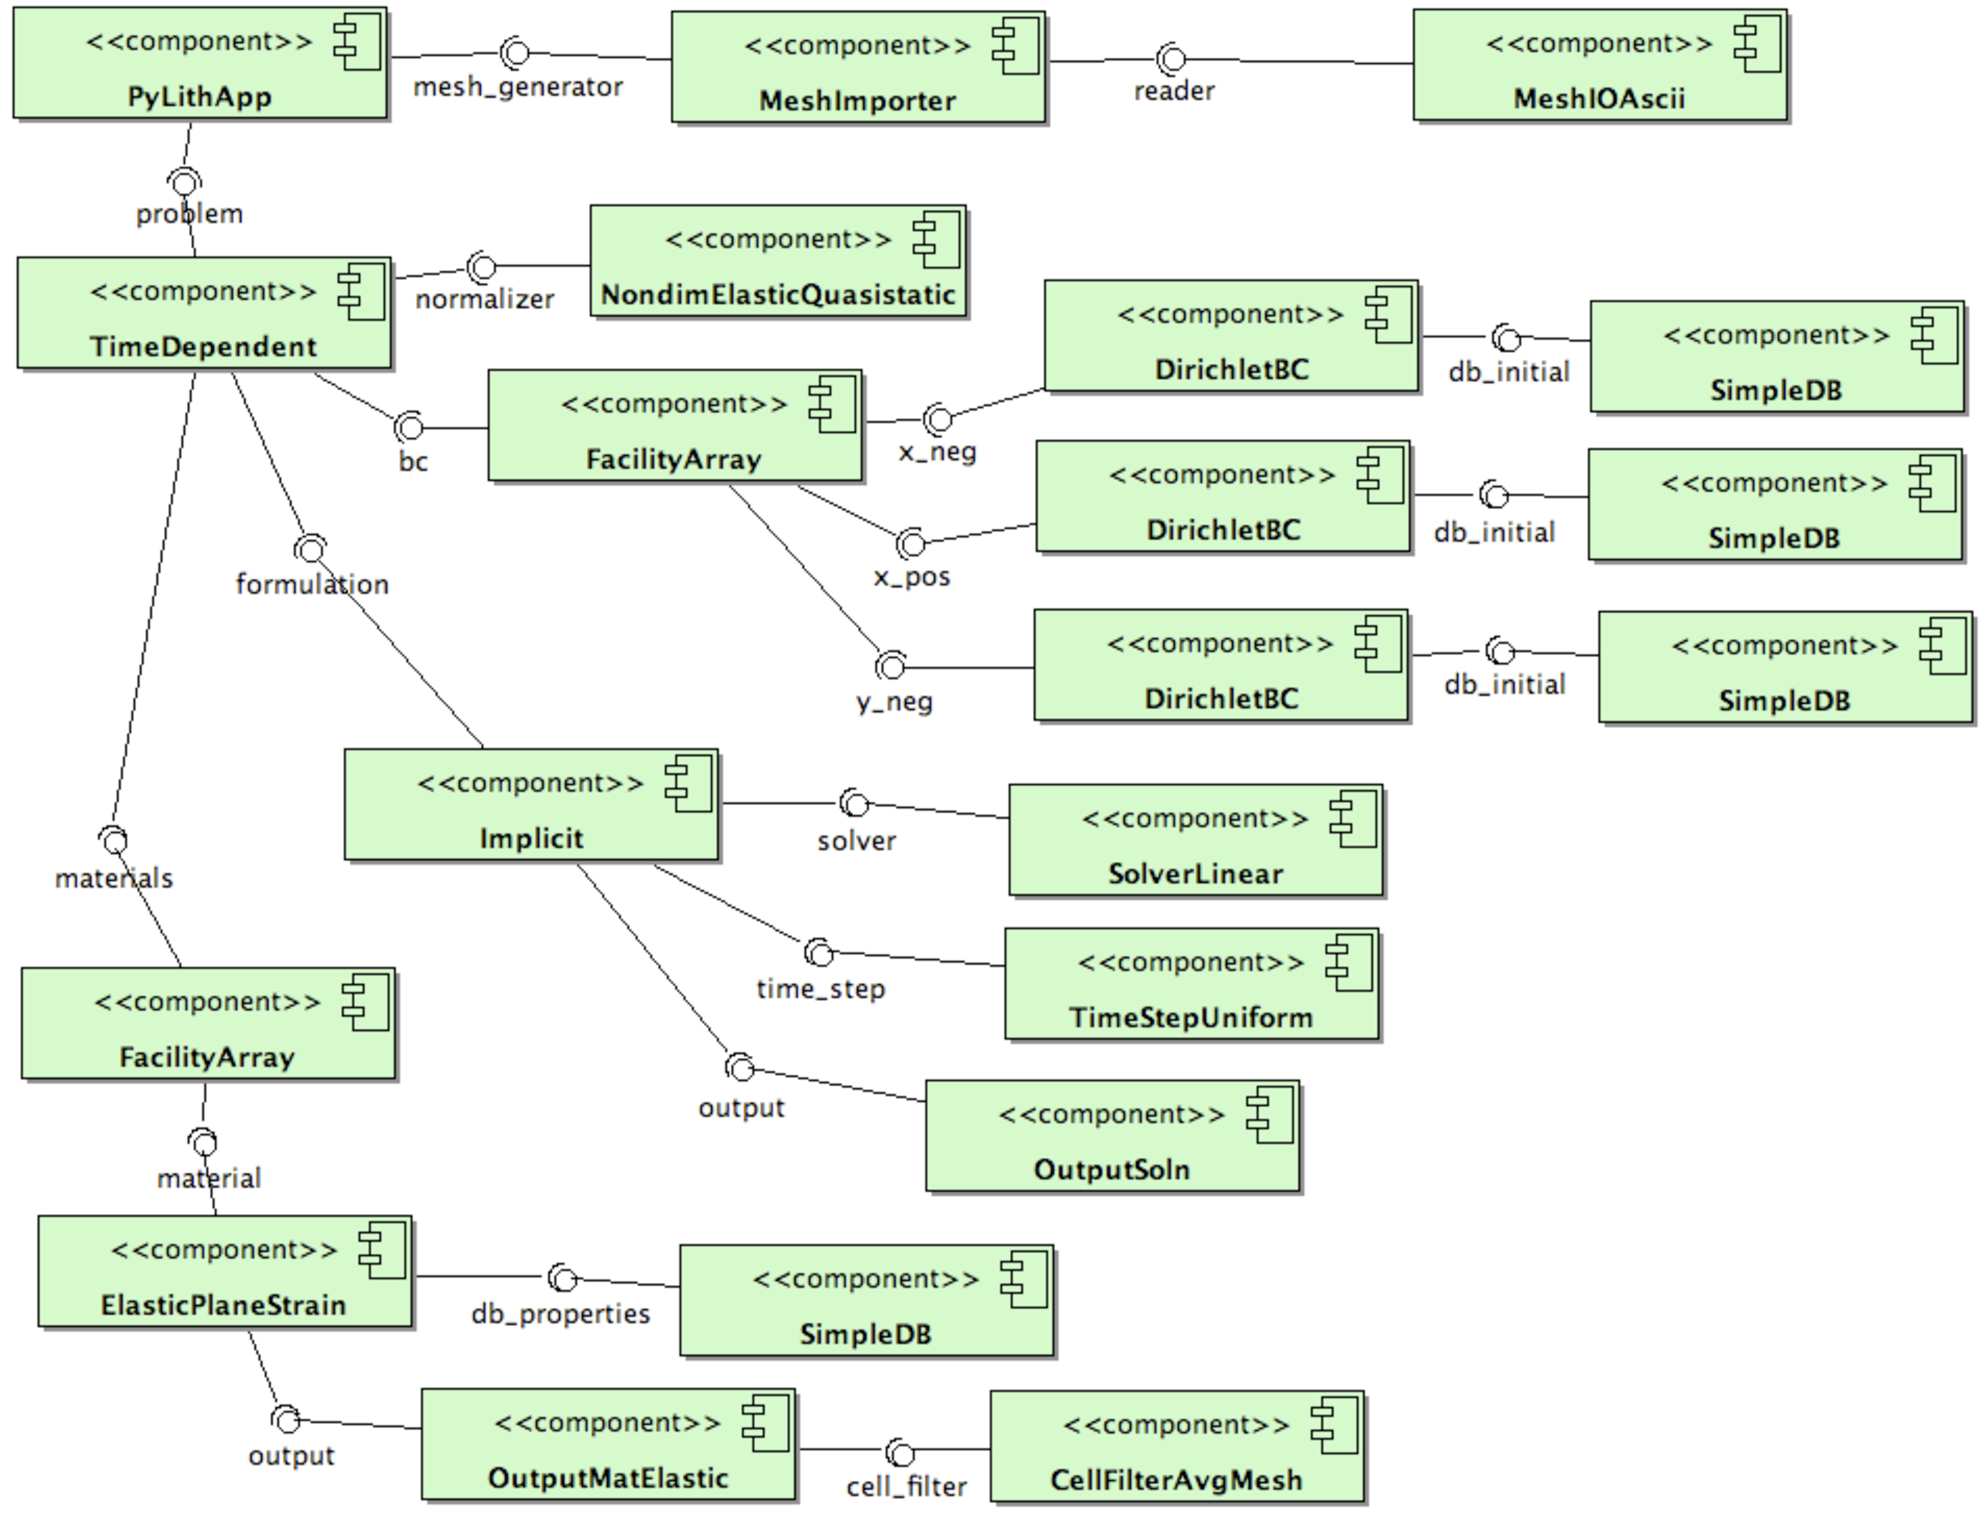
\includegraphics[scale=0.70]{figs/axialdisp}

% ------------------------------------------------------------ SLIDE
\foilhead{Example: {\tt twocells/twoquad4 axialdisp.cfg}}
  \summary{}

  \begin{minipage}[t]{4in}
    {\centering {\bf Input}}
    \begin{itemize}
    \item Simulation parameters
      \begin{itemize}
      \item {\tt pylithapp.cfg}
      \item {\tt axialdisp.cfg}
      \end{itemize}
    \item ASCII Mesh: {\tt twoquad4.mesh}
    \item Spatial databases
      \begin{itemize}
      \item {\tt matprops.spatialdb}
      \item {\tt axialdisp.spatialdb}
      \end{itemize}
    \end{itemize}
  \end{minipage}
  \hfill
  \begin{minipage}[t]{4.75in}
    {\centering {\bf Output}}
    \begin{itemize}
   \item Displacement field
      \begin{itemize}
      \item {\tt axialdisp\_t000000.vtk}
      \end{itemize}
    \item State variables
      \begin{itemize}
      \item {\tt axialdisp-statevars\_info.vtk} (physical properties)
      \item {\tt axialdisp-statevars\_t000000.vtk} (stress and strain)
      \end{itemize}
    \end{itemize}
  \end{minipage}   

% ------------------------------------------------------------ SLIDE
\foilhead{Example: {\tt 3d/hex8 savageprescott.cfg}}
  \summary{Creep and repeated rupture on a strike-slip fault}
 
\movie{0.5in}{0.0in}{8.0in}{5.7778in}{movies/savageprescott_soln}%


% ------------------------------------------------------------ SLIDE
\foilhead{Example: {\tt 3d/hex8 savageprescott.cfg}}
 \summary{}

{\small
 \hspace*{-0.5in}
  \begin{minipage}[t]{4.5in}
    {\centering {\bf Input}}
    \begin{itemize}
    \item Simulation parameters
      \begin{itemize}
      \item {\tt pylithapp.cfg}
      \item {\tt savageprescott.cfg}
      \end{itemize}
    \item Mesh: {\tt box\_hex8\_1000m.exo}
    \item Spatial databases
      \begin{itemize}
      \item {\tt mat\_elastic.spatialdb}
      \item {\tt mat\_maxwell.spatialdb}
      \item {\tt finalslip\_rupture.spatialdb}
      \item {\tt sliptime.spatialdb}
      \item {\tt sliprate\_creep.spatialdb}
      \end{itemize}
    \end{itemize}
  \end{minipage}
  \hfill
  \begin{minipage}[t]{4.75in}
    {\centering {\bf Output}}
    \begin{itemize}
   \item Displacement field
      \begin{itemize}
      \item {\tt savageprescott\_tNNNN.vtk}
      \item {\tt savageprescott-groundsurf\_tNNNN.vtk}
      \end{itemize}
    \item State variables
      \begin{itemize}
      \item {\tt savageprescott-elastic\_info.vtk}
      \item {\tt savageprescott-elastic\_tNNNN.vtk}
      \item {\tt savageprescott-viscoelastic\_info.vtk}
      \item {\tt savageprescott-viscoelastic\_tNNNN.vtk}
      \end{itemize}
    \item Fault
      \begin{itemize}
      \item {\tt savageprescott-fault\_info.vtk}
      \item {\tt savageprescott-fault\_tNNNN.vtk}
      \end{itemize}
    \end{itemize}
  \end{minipage}   
}

% ------------------------------------------------------------ SLIDE
\foilhead{Useful Tips/Tricks}
  \summary{}

  \begin{itemize}
  \item {\tt pylithinfo [--verbose] [PyLith args]}\\
    Dumps all parameters with their current values to text file
  \item Command line arguments
    \begin{itemize}
    \item {\tt --help}
    \item {\tt --help-components}
    \item {\tt --help-properties}
    \item {\tt --petsc.start\_in\_debugger} (run in xterm)
    \item {\tt --nodes=N} (to run on N processors on local machine)
    \end{itemize}
  \item PyLith User Manual
  \item CIG Short-Term Tectonics mailing list\\
    {\tt cig-short@geodynamics.org}
  \item CIG bug tracking system\\
    {\tt http://www.geodynamics.org/roundup}
  \end{itemize}

% ------------------------------------------------------------ SLIDE
\foilhead{Crustal Deformation Modeling}
  \summary{Overview of workflow for typical research problem}

  \vfill
  \begin{center}
    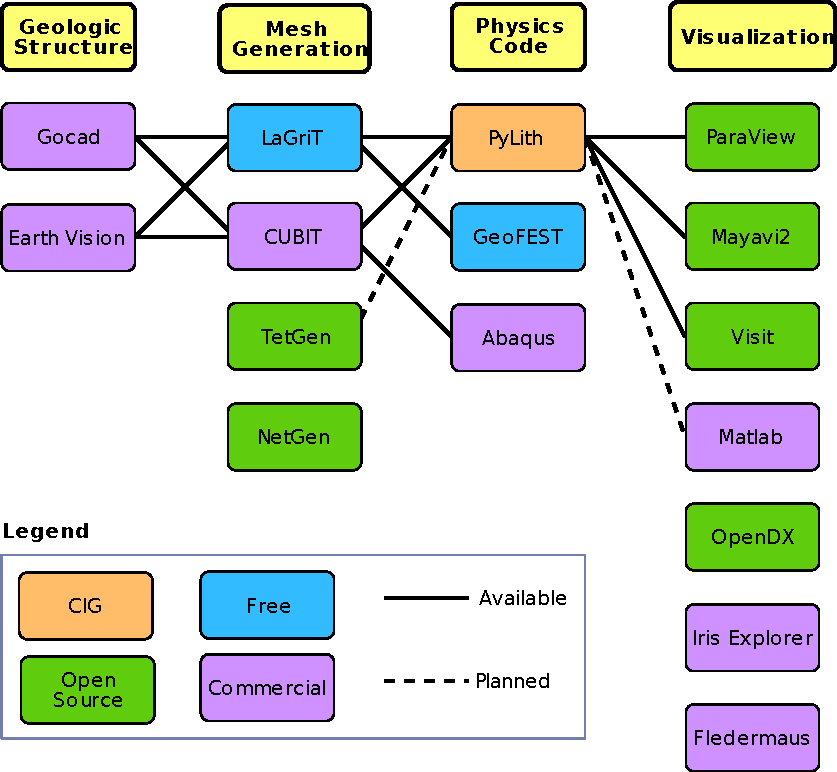
\includegraphics[scale=1.15]{figs/workflow}
  \end{center}
  \vfill


% ======================================================================
\end{document}


% End of file
